\documentclass[notumble,combine]{leaflet}
\usepackage[dvipsnames,usenames]{color}
\usepackage{graphicx}
\usepackage{alltt}
\usepackage{url}
\usepackage{ascmac}
\usepackage{comment}
\usepackage{here}
\usepackage{wrapfig}

\makeatletter
% from leaflet.cls
\renewcommand\section{\@startsection{section}{1}{\z@}%
  {-3.5ex \@plus -.75ex}%
  {1ex} %{1.5ex}%
  {\normalfont\large\sectfont\color{NavyBlue}}}
\renewcommand\subsection{\@startsection{subsection}{2}{\z@}%
  {-2.5ex plus -.5ex}%
  {1\p@} %{1ex}%
  {\normalfont\normalsize\sectfont\color{BrickRed}}}
\makeatother

\graphicspath{{figures/}} 

\title{
	\vfill
	\includegraphics[width=\textwidth]{kbug-logo}
	\vfill
	\resizebox{\linewidth}{!}{\bf 関西*BSDユーザ会}%
	\\[\baselineskip]
        \resizebox{\linewidth}{!}{{\bf \url{http://www.kbug.gr.jp/}}}
	\vfill
        \parbox[c]{3cm}{\resizebox{3cm}{!}{\textcolor{red}{\bf{@}}}}
	\parbox[c]{4cm}{\includegraphics[width=4cm]{kyoto_tower}}\\
	
\includegraphics[width=\textwidth]{logo-kyoto-2011}
        \resizebox{\linewidth}{!}{{\bf \url{http://www.ospn.jp/osc2011-kyoto/}}}\\
        \resizebox{\linewidth}{!}{2011年7月15日(金),16日(土)}
}

\date{}

\begin{document}
\maketitle
\thispagestyle{empty}
\pagebreak{}
\section{関西*BSDユーザ会ってなに?}
関西 *BSD ユーザ会 (Kansai *BSD Users Group; K*BUG)とは、
BSD系OSのユーザ同士の情報交換のための{\em 場}で、1999年に作
成されました。

年に数度の勉強会やイベントの参加、そして宴会を行っています。

\subsection{K*BSDの基本理念}
K*BUGの基本理念は以下のようになっています
(\url{http://www.kbug.gr.jp/charter.html}より)。

\fbox{\begin{minipage}{\textwidth}
\begin{itemize}
\item 場の提供を目的とする
\item 人のケツは叩くが足は引っ張らない
\item 来るものは拒まず、猿ものは追わず
\item だれでも役員になれる。誰でも役員は止められる
\end{itemize}
\end{minipage}}
\begin{wrapfigure}[8]{r}{3cm}
\begin{center}
 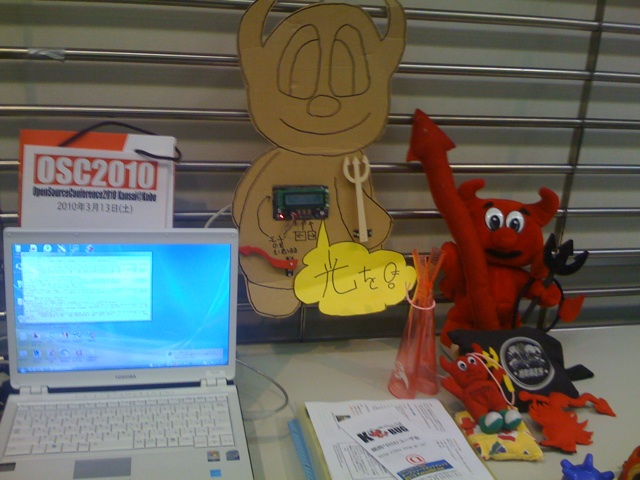
\includegraphics[width=3cm]{74251436}\\
\end{center}
\end{wrapfigure}

少し難しく感じるかもしれないですが、\textcolor{red}{BSDへの愛と情熱}があれば、
あなたが\textcolor{blue}{やりたいと思うことができる場}がK*BUGなのです。

また、メンバーは色々な技術に詳しいですし、技術に関する話も大好きなので、
あなたの疑問などもぶつけてみてください。

\section{最近の活動}
最近の活動とその内容は以下のとおりです。

もし、興味のあるテーマがあるようでしたら、是非一度遊びにきてください。

\subsection{2011年6月18日(土)@京都 第2回研究会}
\begin{itemize}
\item 小ネタ3つ: mount\_smbfsではまった話、\\
  mount\_smbfs / fuse\_smbnetfsが遅い、\\
  10日に1回panicする話 % by 野田
\item LTEのドライバー % by わたなべ
\item pkgsrc-2011Q2について % by taca
\item What Operating System Has Crashed Here? % by かわもと
\item OpenSSHの謎を学ぶ % by かわもと
\item Interactive shell for blockdiag \\ http://interactive.blockdiag.com/ の可能性
\item 懇親会@んまい
\end{itemize}

\subsection{2011年4月16日(土) in OSC2011 Kansai@Kobe}

\subsection{2011年2月19日(土)@大阪 第1回研究会+新年会}

\subsection{2010年12月11日(土)@京都 定期総会+第6回研究会+忘年会}
\begin{itemize}
\item 定期総会
\item RockTubeのファーム % by 西東
\item ZFS Rootのはまりどころ % by 寺本
\item DNSSEC 対応レゾルバを10分で用意する % by umq
\item freebsd-updateで7.1からupgradeしてみた % by umq
\item clang/LLVMの小ネタ % by umq
\item 夏の怪談その後 (diskが治った!!) % by かわもと
\item KOF2011 K*BUGブース報告 % by いしはら
\end{itemize}

\subsection{2010年11月5日(土)-6日(日) in KOF2010}
ユビキタスなK*BUGの祭典。
\begin{itemize}
\item NetBSD/xen (Dom0)で\{Net, Open, DragonFly\}BSD (DomU)
\begin{itemize}
 \item Live on air!! CentOS and Gentoo/Dragonfly  (DomU)
 \item FreeBSD (DomU) is not work orz.
\end{itemize}
\item OpenBSD/landisk on USL-5P で Active/Stanby FW (pf + CARP)
\item OpenBSD/zaurus by NBUG
\item Song with us, OpenBSD release songs!! (endless)
\item 64bitの20年 at 中村ブース (K*BUGメンバー)
\item LinuxでDAW  at 中村ブース (K*BUGメンバー)
\end{itemize}

\subsection{2010年9月11日(土)@京都 第5回研究会}

\subsection{2010年7月24日(土)@神戸 第4回研究会}

\subsection{2010年7月9日(金),10(土) in OSC2010 Kansai@Kyoto)}
\begin{itemize}
\item NetBSD/sandpoint(かわうち版) 4\_STABLE on LinkStation
\item DragonFlyBSD/i386 2.6.3 on MURAMASA
\item OpenBSD/landisk 4.7 on USL-5Pでe-mobileルータ
\item FreeBSDのX環境を22分で構築する % by 野田
% \item [JNUG] WZero3 + 2GB over SDで、何かが起こる…
\end{itemize}

\subsection{2010年5月15(土)@京都 第3回研究会}
葵祭の日に何かが起こる…
\begin{itemize}
\item ArecXの話 % by 西東
\item SDIOな無線LAN % by 渡辺
\item syslog(3)話 % by 神戸
\item SDIOの話、再び % by 渡辺
\item ハードディスク買いました % by 西東
\item aristanetworks.comの話 % by 安田
\end{itemize}

\section{BSDに関する情報}
\subsection{BSD開発元リンク (日本語情報)}
\begin{itemize}
\item NetBSD情報 by JNUG\\
  \url{http://www.jp.netbsd.org/}
\item FreeBSD友の会  \url{http://www.jp.freebsd.org/}
\item OpenBSD本家  \url{http://www.openbsd.org/ja/}
\item DragonFly BSD \url{http://dragonflybsd.org/}
\end{itemize}

\subsection{ご近所BSDユーザ会リンク}
\begin{itemize}
\item JNUG(Japan NetBSD Users Group)\\
  今回もお隣でブースをさせてもらいました\\
  \url{http://www.jp.netbsd.org/ja/JP/JNUG/}
\item 名古屋*BSDユーザグループ \\ \url{http://www.nagoya.bug.gr.jp/}
\item 四国*BSDユーザ会 \\ \url{http://flathill.gr.jp/sbug/}
\end{itemize}

\newpage
\subsection{K*BUG関連}
以下のようなURLで、メンバーの活動が紹介されていますので、参考にしてください。

\begin{minipage}{\textwidth}
\begin{shadebox}
\begin{itemize}
 \item Twitter \url{http://twitter.com/610t/kbug}
 \item いしはら \url{http://www.tunagu.gr.jp/fswiki/isihara/}
 \item うえだ \\ \url{http://www.ueo.co.jp/~tueda/diary/}
 \item 西東 \url{http://d.hatena.ne.jp/tunefs/}
 \item 白井 \url{http://hp.vector.co.jp/authors/VA012337/misc/presentation.html}
 \item たけおか \url{http://www.takeoka.org/}
 \item 寺本 \url{http://d.hatena.ne.jp/mteramoto/}
 \item むとう \url{http://qml.610t.org/FreeBSD/}
 \item 野田 \url{http://d.hatena.ne.jp/akira_you/}
\end{itemize}
\end{shadebox}
\end{minipage}

\section{これからの関連イベント(予定)}
K*BUGでは、だいたい2ヶ月に1度の頻度で勉強会を行っています。
また、主に関西のイベントで、展示などを行っています。

現在、予定されているイベントは、以下のとおりです。
詳細に関しては、K*BUGのWebページをご確認ください。

\begin{itemize}
\item 2011年8月20日(土) 第3回研究会@京都
\item 2011年10月15日(土) 第4回研究会@大阪
\item 2011年11月11日(金)-12(土) KOF2011@大阪
\item 2011年12月10日(土) 定期総会+第5回研究会+忘年会@大阪
\end{itemize}

\newpage
\section{K*BUG in OSC2011 Kansai@Kyoto}
祇園祭に負けないくらい、あつい二日がそこに…
\subsection{展示: 驚くほどたくさんの○○BSDが…}
\begin{itemize}
 \item NetBSD/xen (Dom0) で、 \{Net, Free, Open, DragonFly\}BSD (DomU)
 \item 組み合せ爆発: \{Free,Net\}BSD × Squeak / Processing × Gainer / Arduino × 木彫
\end{itemize}

\subsection{NetBSDのご紹介 by JNUG}
以下のように「NetBSDのご紹介」を行いますので、ご参加ください。

\begin{itemize}
\item 日時: 2010/07/15(金) 15:15-16:00
\item 会場: 小会議室C
\item 講師: 蛯原 純 (The NetBSD Project/株式会社創夢)
\item 主催:日本NetBSDユーザーグループ
\item 対象者:オペレーティングシステム/組み込み機器/ワークステーション/WZero3に興味がある方。
\item レベル:初級〜中級者向け
\item \url{https://www.ospn.jp/osc2011-kyoto/modules/eguide/event.php?eid=1}
\end{itemize}

NetBSDは、自由に利用可能で、BSDライセンスに基づき再配布可能なUNIX-likeオペレーティングシステムです。NetBSDの概要および最近の動向をご紹介します。

\begin{comment}
BSD系UNIXを取り巻く環境と、将来の展望について議論し、 BSDコミュニティ間の情報交換を行なうBOFセッションです。
4.4BSDの流れをくむFreeBSD/NetBSD/OpenBSDなど、 BSD系UNIXのユーザグループ合同で、BSD系UNIX全般を対象とした幅広いテーマで議論します。
\end{comment}

\vfill

\begin{minipage}{\textwidth}
\begin{boxnote}

\section{kbug-usersメーリングリスト}
K*BUGでは、K*BUGメンバーの情報交換や、イベントなどの情報伝達用に
kbug-usersメーリングリストを用意しています。

K*BUGメンバーは、基本的にはこのメーリングリストを読んでいることが期待
されます。

購読は以下のURLをご参照ください。

 \url{http://www.kbug.gr.jp/maillist.html}
\end{boxnote}
\end{minipage}

\end{document}  
